\chapter{Implementation}%%%%%%%%%%%%%%%%%%%%%%%%%%%%%%%%%%%%%%%%%%%%%% 
\label{chap:implementation}
This section presents the (software) implementation details of the methodology.

First, \refsec{sec:implementation:representation}.
Second, \refsec{sec:implementation:compilation}.
Then, \refsec{sec:implementation:loading}.
Finally, \refsec{sec:implementation:utilization}.

\section{\mySubRQOneTitle: The Geofront Application}

\begin{figure}
  \centering
  \graphicspath{ {../../assets/images/implementation/} }
  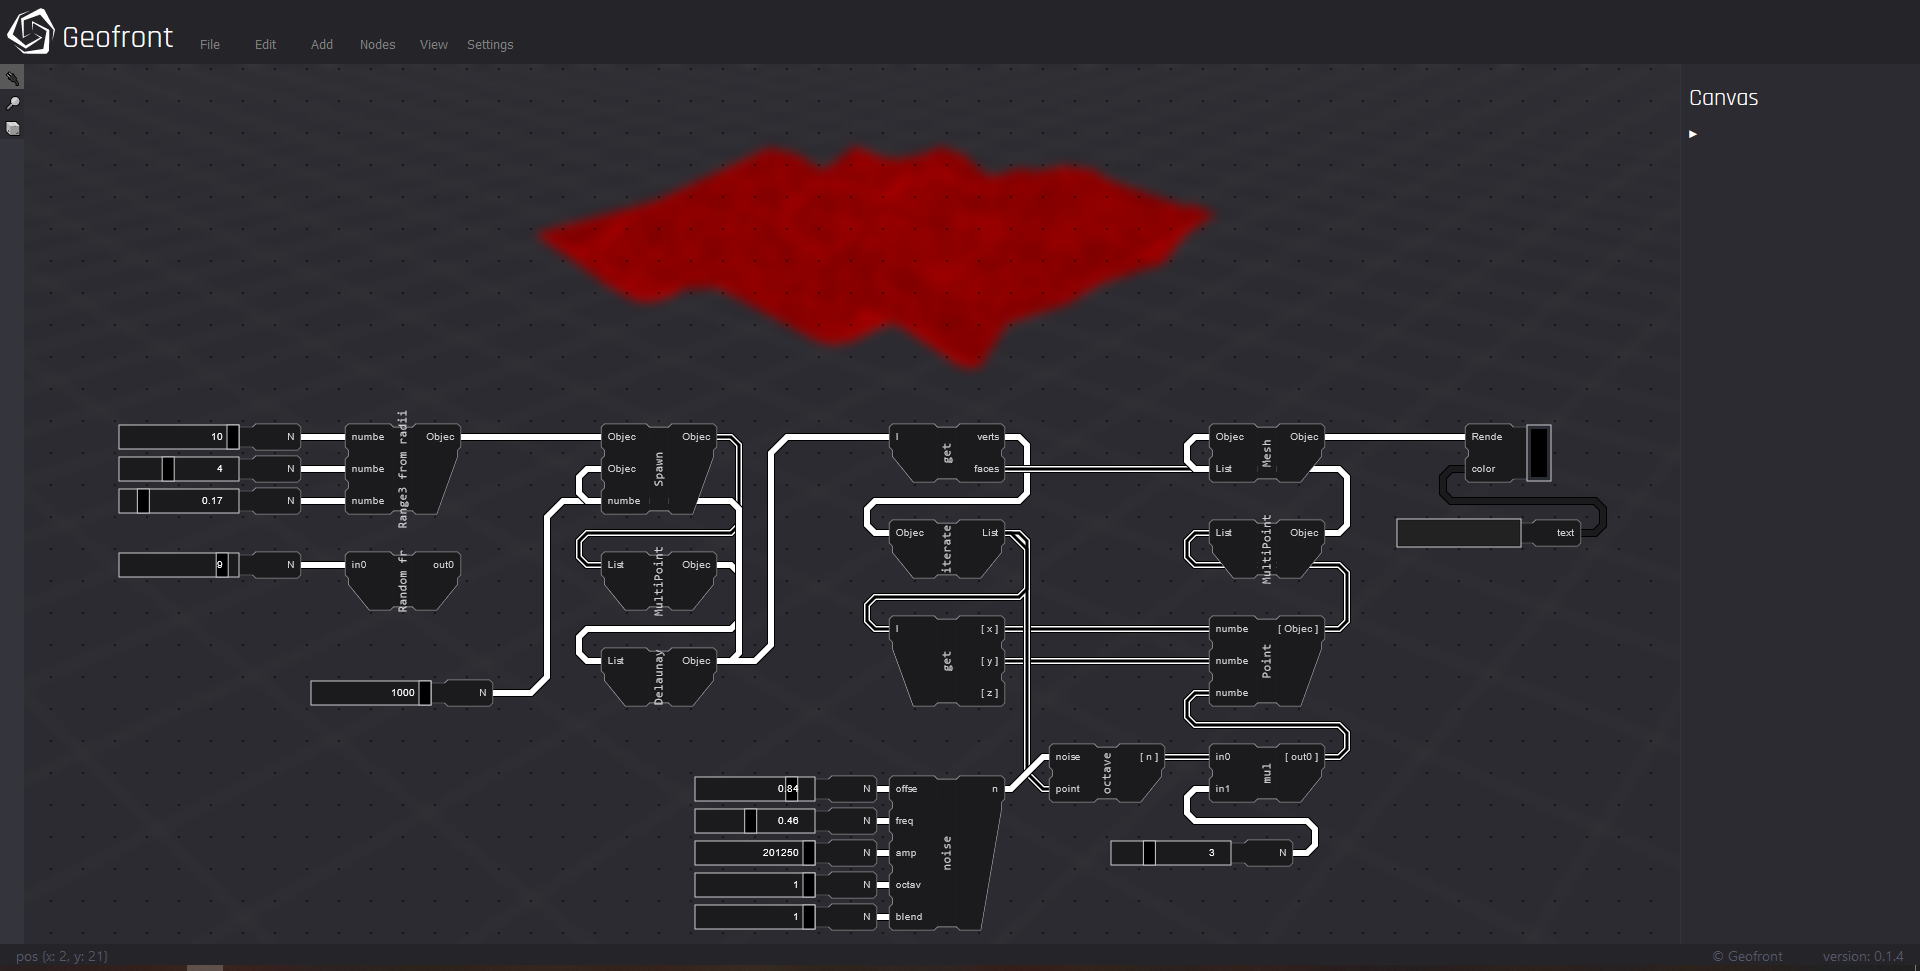
\includegraphics[width=\linewidth]{full-application.png}
  \caption[Geofront]{The Geofront Application}
  \label{fig:geofront-app}
\end{figure}

\label{sec:implementation:representation}
To implement the component of \mySubRQOneTitle, the core of the prototype application had to be created.
To the best of the authors knowledge, no web-based dataflow-VPL project could be found to serve as a starting point. 
This is why the full application had to be created from scratch (actual scratch, not to be confused with the scratch language: (SOURCE: SCRATCH LANGUAGE)). 

This section explains the significant components of this prototype application. 
The prototype is titled "Geofront", as a concatenation of "geometry" and "frontend".

% Explain main code setup \& components
Geofront exists as a set of loosely coupled repositories, all published on the version control platform GitHub under the MIT license. These repositories are grouped under the GitHub Organization \m{thegeofront} : https://github.com/thegeofront .
The \m{app} repository holds the main Geofront application. It contains the source code for most aspects, such as the basic UI, the visual programming interface, and the standard components. The application is hosted at (https://thegeofront.github.io/).
The \m{engine} repository is the library used for the 3D visualizations, some of the logic within the graph components, and some helper functions.
The repositories prefixed with a \m{gfp} are Geofront Plugins. These plugins are consumed by the main \m{app}.

The Geofront Application (\m{app}) is set up using a \m{TypeScript} codebase. It uses \m{webpack} to compile this to a singular javascript file, and this file practically represents the full application. 
the repository used around 9.000 lines of code, divided into core categories and functionalities:
\begin{enumerate}[I]
  \item \m{shims}: Models to reason about 'programming language features', such as functions and variables.
  \item \m{nodes-canvas}: Contains the model, renderer and controller of the visual programming graph itself.  
  \item \m{modules}: holds all classes dedicated to dynamically loading plugins.
  \item \m{std}: The default plugin, baked into Geofront.   
  \item \m{html}: a 'web framework' of reusable html components making up the UI visuals.
  \item \m{menu}: a menu system which takes care of the model \& logic of the UI.
  \item \m{viewer}: The 3D renderer accompanying Geofront.
  \item \m{util}: Utility functions.   
\end{enumerate}
What follows is a clarification of some of these categories.

\subsection{Shims}

\begin{figure}
  \centering
  \graphicspath{ {../../assets/images/implementation/} }
  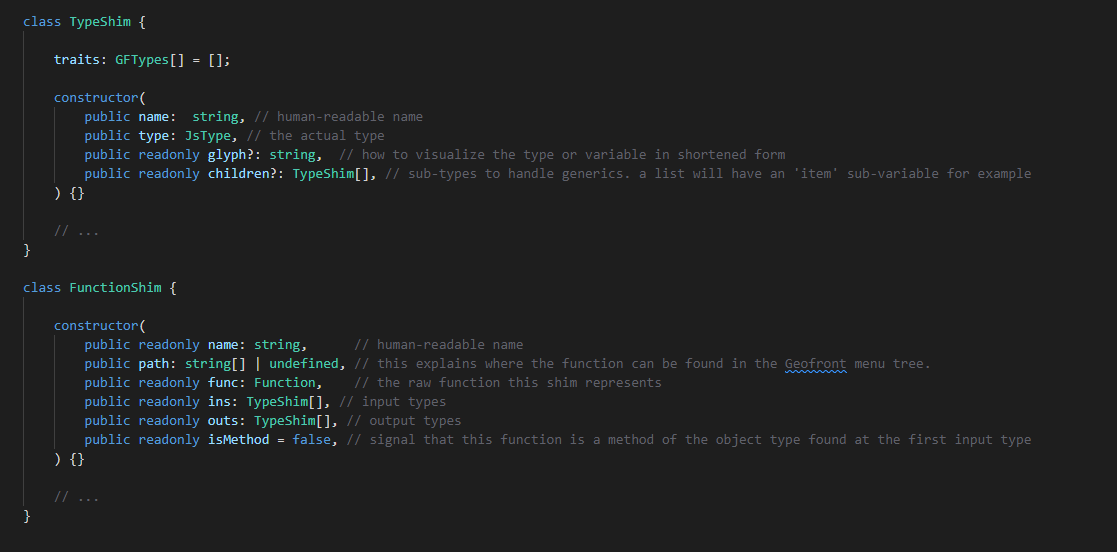
\includegraphics[width=\linewidth]{shim-uml.png}
  \caption[Shim Classes]{}
  \label{fig:shim-classes}
\end{figure}

Since Geofront is partially a programming language, a way was needed to reason about some of the features of a programming language, such as functions, types, variables, and modules / libraries / plugins. 
This is why the \m{FunctionShim}, \m{TypeShim}, \m{VariableShim} and \m{ModuleShim} classes exist, respectively (see \reffig{fig:shim-classes}). 
For example, the \m{FunctionShim} offers the name, description, number of inputs, and number of outputs of a function, as well as ways to invoke the function it represents.
These inputs and outputs have corresponding \m{TypeShims}, which are formal representations of TypeScript / JavaScript-based types. 
TypeShims can be structured recursively to define a \m{List of List of strings} for example. The \m{TypeShim} is also used to reason about type checking and type compatibility.

the shims are a set of classes used in almost all other categories within Geofront. 
The shim classes are designed using the Object Type design pattern (SOURCE: BIG FOUR). 
In short, this means that one function corresponds to exactly one \m{FunctionShim} instance, and that this instance is shared with any object wishing to use the function. 
The name \m{shim} was taken from \m{wasm-bindgen}'s (SOURCE) naming convention for the auto-generated \m{JavaScript} and \m{TypeScript} files. These classes were first created as a representation of those shims.


\subsection{Nodes Canvas}
From the Shim models, the main model of the visual language can be constructed. 
The \m{nodes-canvas} category contains all logic \& visualization of the visual programming graph, and writing this category was equivalent to developing the visual programming language itself. 
The other categories of the repository can be understood as auxiliary to this one.

\subsubsection*{Representation}

% TODO uml diagram?
% Picture of a single node
% Picture of a single cable

The architecture of Geofront's visual programming language is first and foremost a Model View Controller setup. 
The Model is at its core a Directed Acyclic Graph (DAG). 
This DAG is an object-oriented, graph-like representation of the data flow of a regular programming language. 

This architecture is implemented using multiple classes. The Viewer and Controller are represented by the \m{NodesCanvas}, which has access to a \m{Graph} Model, containing \m{Nodes} and \m{Cables}. 

Nodes are analogous to the "Functions" of normal programming languages. 
As such, a Node knows about the function they invoke through a \m{FunctionShim} reference. 
The node contains a number of input and output sockets based on this information, and each socket contains exactly one optional reference to a \m{Cable} (SEE PICTURE).  
As the name implies, these Nodes form the nodes of the DAG. However, they differ from a pure DAG implementation, in that they also provide pointers back in the reverse direction, forming essentially a normal graph, or a doubly linked list. 

The Cables are \geofront{}s analogy to normal "Variables". Cables know about the type they represent through a \m{TypeShim}. A Cable must have exactly one origin, which is an output socket of a Nodes, and must have one or more destinations, which are the input sockets of other Nodes (SEE PICTURE).

From these ingredients, a graph can be constructed. 
To reason about this graph as a whole, the \m{Graph} class was introduced. 
It contains methods and functions to add or remove nodes, to add and remove cables between nodes, to parse the graph from and to a json, and to calculate the graph.  
This study chose to centralize most logic to this Graph, instead of adding complex logic to individual Nodes. 
This centralized approach was deemed more clear: Many of the required functionalities cover multiple nodes, and this is better presented from an "overview" perspective of theb 
Because of the way Cables and Nodes reference each other, the graph has characteristics of a doubly linked list data structure. Using normal references in these types of situations could easily lead to memory management issues such as Dangling Pointers. Even though the JavaScript runtime is garbage collected, it is still subject to memory leak issues or runtime errors. Substituting references with ids makes it easier to prevent these types of problems. 
% does not solve all problems automatically

Finally, this entire graph object is accessed by a larger \m{NodesCanvas} object, and this canvas has the responsibilities of "View" and "Controller". 

\subsubsection*{RenderingE}

\begin{figure}
  \centering
  \begin{subfigure}[b]{0.30\linewidth}
    \graphicspath{ {../../assets/images/implementation/} }
    \centering
    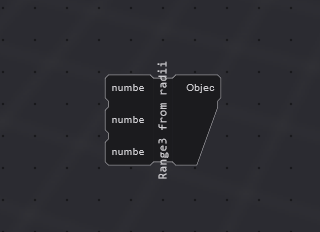
\includegraphics[width=\linewidth]{node.png}
    \caption{}\label{fig:node-cable:1}
  \end{subfigure}%
  \qquad 
  \begin{subfigure}[b]{0.30\linewidth}
    \graphicspath{ {../../assets/images/implementation/} }
    \centering
    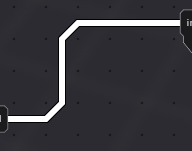
\includegraphics[width=\linewidth]{cable.png}
    \caption{}\label{fig:node-cable:2}
  \end{subfigure}%
  \qquad 
  \begin{subfigure}[b]{0.30\linewidth}
    \graphicspath{ {../../assets/images/implementation/} }
    \centering
    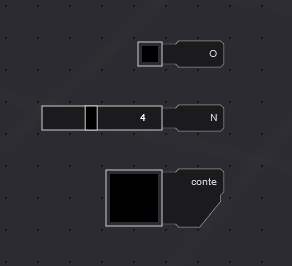
\includegraphics[width=\linewidth]{widgets.png}
    \caption{}\label{fig:node-cable:3}
  \end{subfigure}%
  \caption[Nodes, Widgets and Cables]{The basic canvas components of Geofront: a Node (A), a Cable (B), and some Widgets (C) }
  \label{fig:node-cable}
\end{figure}

This nodes data model must be rendered to the screen so users can comprehend and edit the graph. 
This visualization is achieved by using the \href{https://developer.mozilla.org/en-US/docs/Web/API/Canvas_API}{HTML5 Canvas Api}. 
The Canvas API is a raster-based drawing tool, offering an easy to use, high-level api to draw 2D shapes such as lines, squares, circles, and polygons. 
The Nodes Canvas uses this API to draw polylines and polygons at runtime, to represent the cables and nodes respectively. 
These basic shapes and their styles change dynamically, based on features like the length of a cable, how many input sockets a node requires, or whether or not a node is selected. 

Like other HTML5 features, the main advantage is that this API is included and implemented within the browser itself. This method is fast thanks to its C++ based implementation, and can be used without the need to include anything within the source code of the application.

The disadvantage of the Canvas API is that it uses many CPU-based draw calls. it is primarily CPU based, Making it much less fast and efficient than WebGL for instance, which is based on the GPU. 
This is quickly noticeable within interactive applications which need to redraw often, such as Geofront. 
The Canvas is refreshed and redrawn often, and does not distinguish between unchanged and changed features. 
This comes down to a performance linear to the amount of nodes and cables drawn. For the current implementation and scale of Geofront, this performance is acceptable. 

\subsubsection*{ Style }

\begin{figure}
  \centering
  \graphicspath{ {../../assets/images/implementation/} }
  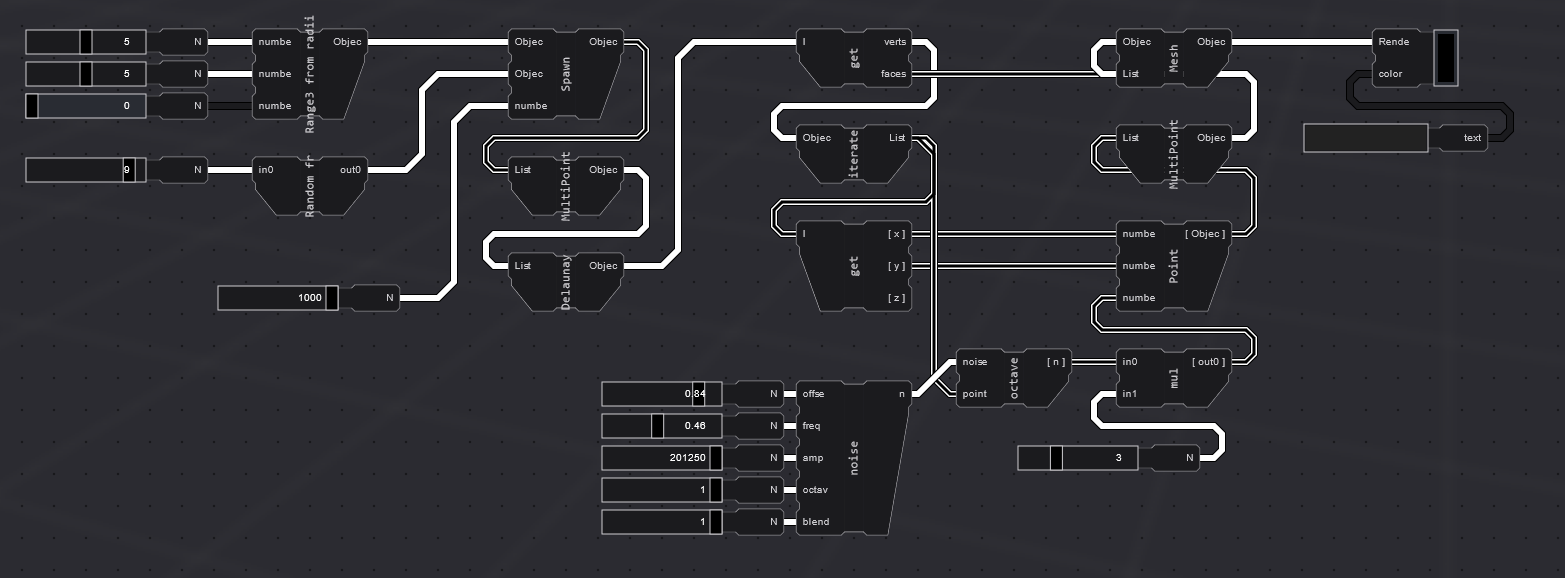
\includegraphics[width=\linewidth]{a-full-graph.png}
  \caption[Shim Classes]{A complete Geofront Script}
  \label{fig:a-full-graph}
\end{figure}

Special care has been put into the stylization of the graph.
The visuals take inspiration from various geometry VPLS, such as Blender's GeometryNodes, McNeel's Grasshopper, and Ravi Peter's GeoFlow (SOURCES). 
A few notable exceptions, however. 
Firstly, the entire graph is placed on a grid, and all nodes strictly adhere to this grid (see \reffig{fig:a-full-graph}). 
For example, a node with three inputs will always occupy three grid cells in height. 
This grid is applied for much of the same reason as terminals \& source code are displayed using monospaced fonts. 
Consistent sizing encourages organization and clarity, for this makes it easy for components to line up, and predict how much space something requires.  
Cables also adhere to the grid. They alter their shape in such a way to remain as octagonal as possible, as an attempt to make connections between nodes more readable.
This takes some additional inspiration from subway maps, as well as the design of computer chips. This makes for a good fit, since both these spatial configurations and the Geofront Script are focussed on organizing connectivity.

\subsubsection{ Interaction }
User Interaction is made possible through the \href{https://developer.mozilla.org/en-US/docs/web/api/event}{HTML DOM Events}. 
This api provides ways to listen to many events, including keyboard and mouse events. 
When the mouse is moved, its screen-space position is transformed to a grid position, which allows the user to select one or multiple objects. 

Geofront's user interface strives to match features of regular desktop applications. 
As such, the Geofront Graph supports features like undoing, redoing, duplication, copying, and pasting. 
These functionalities can be used with the expected keyboard combinations (Ctrl + C / Ctrl + V).

\subsubsection*{ Graph Manipulation }

In order to support these features, especially undo / redo support, we are required to explicitly track the history of the graph. 
This is why a Command Pattern (Big Four, SOURCE) was implemented.
Instead of directly editing the graph, all actions are represented by \m{Action} objects. 
Each Action can 'do' and 'undo' a specific action, and the data needed to make this do and undo are stored within the action. 
By then introducing a bridge class we decouple the graph and controller, only allowing interaction with the graph by giving this bridge Action objects. The Bridge maintains a stack of undo and redo actions, which represents this history.  

% Additionally, editing any graph data structure is never trivial. 
% Special care must be taken to ensure the validity of a graph before and after changes, and is especially the case with Geofront's Doubly linked graph. 
% To the best of the authors knowledge, these is no "trick" or "pattern" to ease this. Instead, the Graph and Graph Decoupler classes both have been designed in such a way 

\subsubsection*{Calculation}

When regarding the Geofront graph, or any other programming language, we see many functions requiring variables which are the result of other functions. 
This is why a graph like this can also be called a dependency graph. 
If we wish to calculate the result of the graph, these dependencies must be taken into account. 
We must sort the functions the graph in such a way that all dependencies are known before a function is calculated.
This problem is known as a topological sorting problem, and can be solved using Kahn's algorithm (\refsec{fig:kahn}): 

\begin{figure}
  \centering
  \begin{lstlisting}
    Step -1: 
      Make an `order` list
    Step 0: 
      Make a `visisted` counter, initialized at 0
    Step 1: 
      Make a `dependency` counter for each node, initialized at 0
    Step 2: 
      Add 1 to this counter for each input edge of this node.
    Step 3: 
      Fill a queue with all dependency 0 nodes. 
      These are the starter nodes.
    Step 4: 
      Remove a node from the queue (Dequeue operation) and then:
      add the nodes' id to the `order` list.
      Increment `visisted` counter by 1.
      Decrease `dependency` counter by 1 for all dependent nodes.
      If one `dependency` counter reaches 0, 
        add it to the queue.
    Step 5: 
      Repeat Step 4 until the queue is empty.
    Step 6: 
      If `visisted` counter is not equal to the number of nodes, 
        then the graph was degenerate, and probably cyclical. 
    \end{lstlisting}
  \caption[Kahns algorithm]{Khan's algorithm in pseudo code}
  \label{fig:kahn}
\end{figure}

Using this algorithm for calculation has several important qualities. 
First of all, it detects cyclical graph patterns without getting trapped within such a loop. 
Graphs implemented on the basis of an event-system suffer from this drawback, and models like these must continuously check their own topology to avoid loops. 

Secondly, by sorting the \emph{order} of calculation before actually performing the calculations, we can use the algorithm for more than just the calculation.
It was this aspect which enabled an earlier version of Geofront to compile a Geofront Script to Javascript at runtime (see \reffig{fig:early-geofront-compile-to-js}).

Finally, if all intermediate calculation results are cached, this same algorithm can also be used for performing partial recalculations of the graph. 
The starting positions of the algorithm then simply become the altered parameter, after which only the required functions will recalculate. 

\begin{figure}
  \centering
  \graphicspath{ {../../assets/images/implementation/} }
  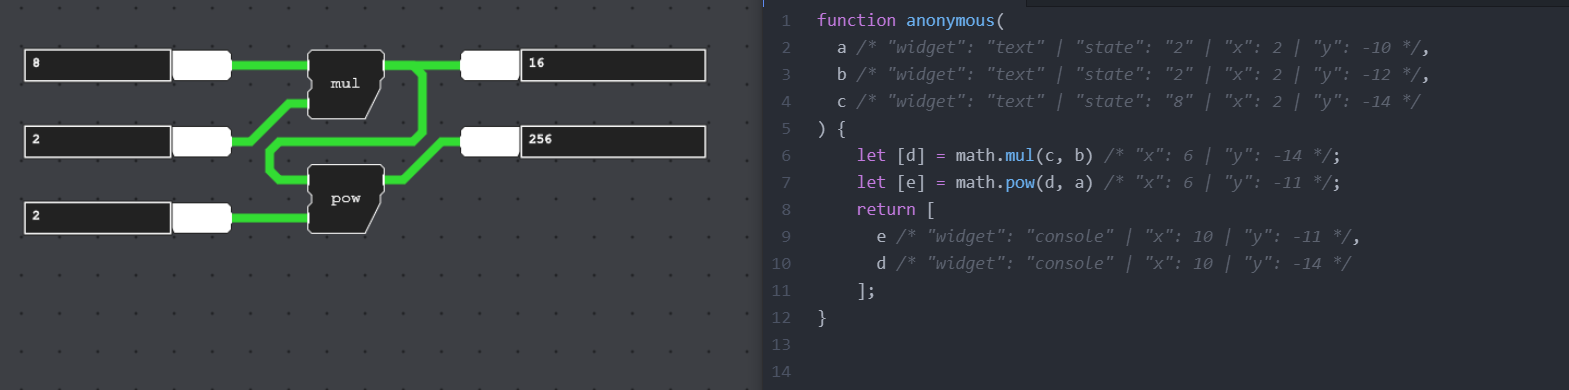
\includegraphics[width=\linewidth]{early-geofront.png}
  \caption[Geofront to js]{An early build of geofront, showing compilation to javascript}
  \label{fig:early-geofront-compile-to-js}
\end{figure}

% \subsection{V. Menu}
% Web Framework

% Every web application requires some amount of html and css to make up its content, and \geofront{} is no exception. 

% \m{html} 

% - No Framework
% - Web Components
% - Typesave Events -> needed, because of the Lapsed listener problem.
% - Webpack + Typescript

% "...
% WebComponents have not been used just as a curiosity. 
% The Graph is intended as a sequence of containerized processes, 
% which whould match WebComponents containerized nature perfectly, just like it matches WebAssembly
% ..."

% with these html components, the basics of the webapp can be created: menu's side menu, and the two main canvases: the graph canvas, and the viewer canvas 
% \geofront{}s use-case is, however, slightly different. We wish to use html as a type of IMGUI. Several cur

\subsection{3D Viewer}

\begin{figure}
  \centering
  \graphicspath{ {../../assets/images/implementation/} }
  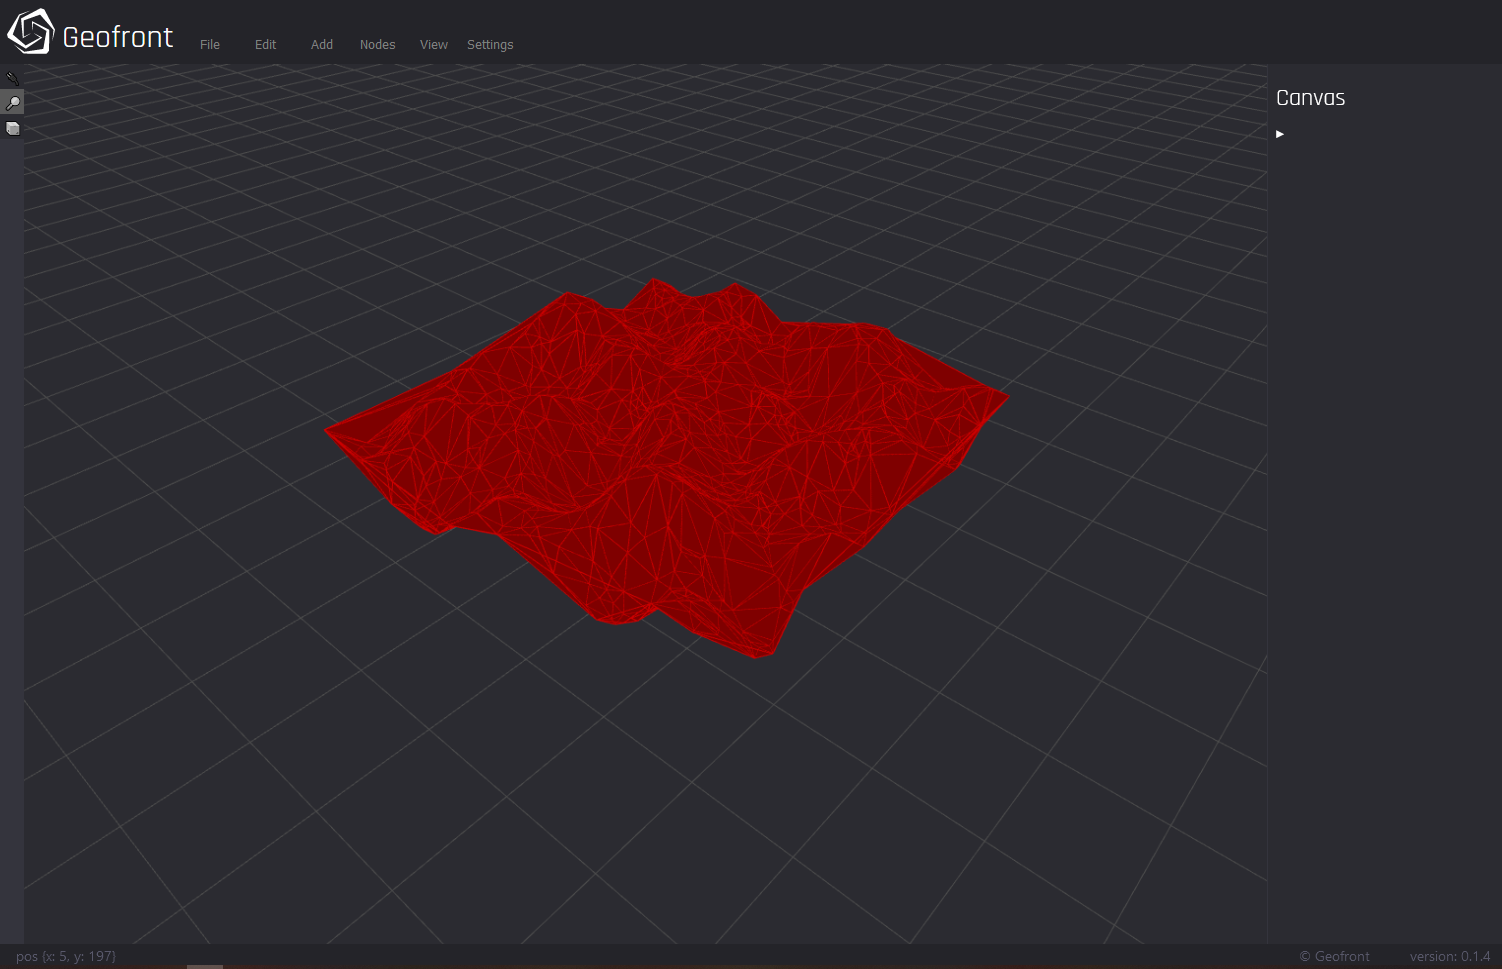
\includegraphics[width=\linewidth]{viewer.png}
  \caption[Geofront viewer]{The Geofront Viewer}
  \label{fig:geofront-viewer}
\end{figure}

Finally, the VPL requires some way of visualizing 3D geometry, so that in-between products containing spatial data can be viewed. 

This study sought to test the browser itself, rather than to test the functionalities of applications layered on top of it, in order to make benchmarks as 'clear' as possible. 

This is why the application makes use of a 3D engine written from scratch to visualize the geometry. 
It goes beyond the scope of this thesis to explain its implementation details, but it can be seen as similar to Three.js (Source).
It uses WebGL and the OpenGL Shading Language (glsl) as its graphics api. 

The viewer can be used to represent and visualize various geometries, such as points, lines, meshes, bezier curves, and bezier surfaces.
Images can also be rendered, which are represented as a quad mesh with a texture. 

These visualization options open the possibility of visualizing a great number of different geodata types, such as DTM / DSM, GEOtiff, Point clouds, and OGC vector data. 

However, specific visualization convertors are not yet implemented, for these are reliant upon the compilation of existing geocomputation libraries. 

\begin{figure}
  \centering
  \begin{subfigure}[b]{0.45\linewidth}
    \graphicspath{ {../../assets/images/implementation/} }
    \centering
    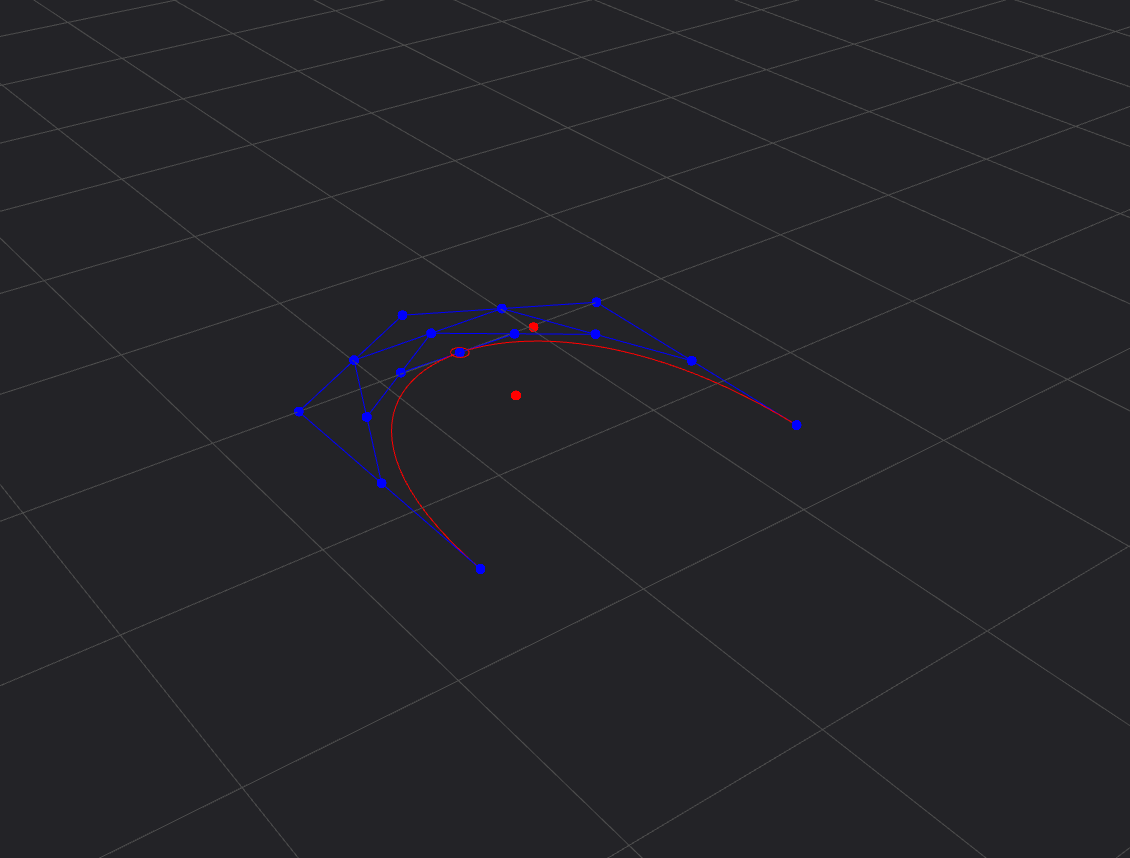
\includegraphics[width=\linewidth]{viewer-2.png}
    \caption{}\label{fig:viewer-geometries:1}
  \end{subfigure}%
  \qquad 
  \begin{subfigure}[b]{0.45\linewidth}
    \graphicspath{ {../../assets/images/implementation/} }
    \centering
    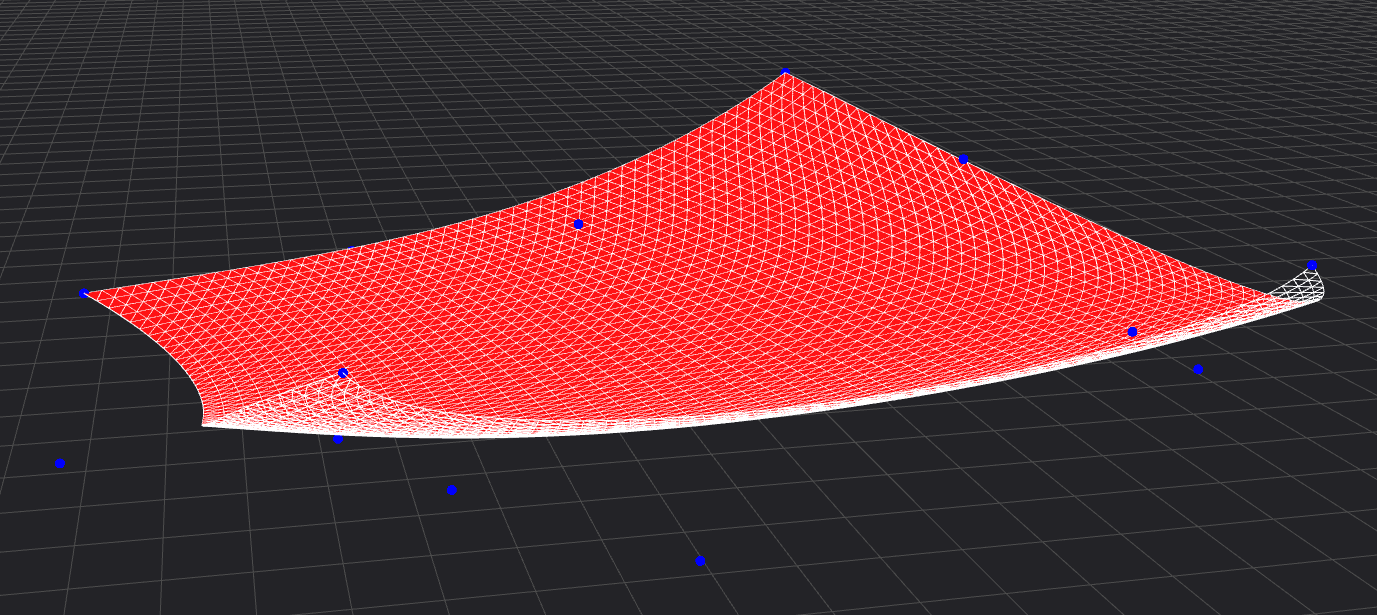
\includegraphics[width=\linewidth]{viewer-3.png}
    \caption{}\label{fig:viewer-geometries:2}
  \end{subfigure}%
  \caption[Geofront viewer geometries]{Some a bezier curve and surface visualized using the geofront viewer}
  \label{fig:viewer-geometries}
\end{figure}

%%%%%%%%%%%%%%%%%%%%%%%%%%%%%%%%%%%%%%%%%%%%%%%%%%%%%%%%%%%%%%%%%%%%%%%%%%%%%%%
%%%%%%%%%%%%%%%%%%%%%%%%%%%%%%%%%%%%%%%%%%%%%%%%%%%%%%%%%%%%%%%%%%%%%%%%%%%%%%%
%%%%%%%%%%%%%%%%%%%%%%%%%%%%%%%%%%%%%%%%%%%%%%%%%%%%%%%%%%%%%%%%%%%%%%%%%%%%%%%

\newpage

\section{\mySubRQTwoTitle: Web-ready geoprocessing libraries}
\label{sec:implementation:compilation}

\subsection{First part}

\begin{note}
TODO write a piece of code in three ways, compare them
\end{note} 

\subsection{Second part}

\begin{note}
Explain the process of taking a C++ / Rust library and putting it onto a web-browser.
\end{note}


\subsubsection*{C++ \& CGAL}

\begin{note}
- sub-dependencies: boost, ..., ...
\end{note}
  
\subsubsection*{Rust \& startin}

\begin{note}
Startin is by no means a replacement of CGAL, 
but it does use robust geometric predicates, and a high precision kernel (f64).
\end{note}

%%%%%%%%%%%%%%%%%%%%%%%%%%%%%%%%%%%%%%%%%%%%%%%%%%%%%%%%%%%%%%%%%%%%%%%%%%%%%%%
%%%%%%%%%%%%%%%%%%%%%%%%%%%%%%%%%%%%%%%%%%%%%%%%%%%%%%%%%%%%%%%%%%%%%%%%%%%%%%%
%%%%%%%%%%%%%%%%%%%%%%%%%%%%%%%%%%%%%%%%%%%%%%%%%%%%%%%%%%%%%%%%%%%%%%%%%%%%%%%

\newpage

\section{\mySubRQThreeTitle: The plugin loader}
\label{sec:implementation:loading}

% _explain how to use webassembly_
% - compiling
% - getting data within webassembly
% - extracting webassembly
% - how to deal with objects? 


% - to turn a function into a component usable in a visual programming graph, lots of meta-data is needed. 
% -> leading to config files 
% -> leading to a barrier between regular programming libraries, and vpl libraries. 
% -> this study opted for automated configs based on 'typescipt' headers to attempt to solve this problem. This worked, but had some new Limitations

The last implementation which requires elaboration is the plugin model. 
A full overview of this system can be given 

% 2 types supported 

% explain advantages & disadvantages of this system. 
Using this system. 



A system for 

...

Using this 


\subsection{ Startin }

\subsection{ CGAL }


\subsection{Assessment}

% [screenshots]

% [show functionalities]

% % ## User Interaction
% % _(basically, write a tutorial)_

\subsection{Within Geofront}



[explain how ]


\subsubsection*{III. Modules} 


The name "Modules" is also used to refer to plugins within the context of \geofront{}.

Shims are automatically created

\emph{explain the system to dynamically load plugins at runtime}

The Dynamic nature of javascript makes it possible tto load plugins at runtime. 

  

\subsubsection{Plugins}
What does a plugin need in order to be acceptable
one javascript file, one type definitions file, and one optional wasm file are accepted. 

ts -> normal build works out of the box
rust -> wasm pack compile target web -> works out of the box 
c++ -> emscripten -> more manual work needed 

\subsubsection{Features}



\subsection{IV. STD / The Standard Library}

The standard library is a 'baked in plugin'.
Points, lines, triangles, vectors, etc.
-> 

Shims are manually created
-> eventually, large parts of the STD can become a plugin


\subsection{Achieved Workflow}
\emph{show the insane (rust + wasm + npm) workflow}

Locally: 
1. Write a geoprocessing / analysis library using a system-level language (rust, C++).
2. Expose certain functions as public, using 'wasm-pack' or 'emscripten'.
3. Compile to `.wasm` + `d.ts` + `.js`.
4. publish to npm (very easy to do with wasm-pack, can also be done with emscripten)

Alternatively: 
1. Write a library using typescript, 
3. Compile to `d.ts` + `.js`.
4. publish to npm 

In Geofront: 
4. Reference the CDN (content delivery network) address of this node package. 


Congrats, this is now a publicly accessible geofront plugin!
The library is loaded, A component is created for each function, with inputs for input parameters, and a singular output. If a 'typescript tuple type' is exported, the plugin loader will create multiple outputs according to each component of the tuple.

- IO can use:
  - basic types (boolean / number / string)
  - jsons, objects, interfaces (typesystem will pick up on them)
  - ArrayBuffers (vital for performant data transfer)



%%%%%%%%%%%%%%%%%%%%%%%%%%%%%%%%%%%%%%%%%%%%%%%%%%%%%%%%%%%%%%%%%%%%%%%%%%%%%%%
%%%%%%%%%%%%%%%%%%%%%%%%%%%%%%%%%%%%%%%%%%%%%%%%%%%%%%%%%%%%%%%%%%%%%%%%%%%%%%%
%%%%%%%%%%%%%%%%%%%%%%%%%%%%%%%%%%%%%%%%%%%%%%%%%%%%%%%%%%%%%%%%%%%%%%%%%%%%%%%
%%%%%%%%%%%%%%%%%%%%%%%%%%%%%%%%%%%%%%%%%%%%%%%%%%%%%%%%%%%%%%%%%%%%%%%%%%%%%%%
%%%%%%%%%%%%%%%%%%%%%%%%%%%%%%%%%%%%%%%%%%%%%%%%%%%%%%%%%%%%%%%%%%%%%%%%%%%%%%%

\section{\mySubRQFourTitle: Utilization}
\label{sec:implementation:utilization}

\begin{note}
  TODO: I might want to add some example applications. 
  Then those will be added here. 
\end{note}